\documentclass{article}
\usepackage[utf8]{inputenc}
\title{MATH 20C Notes - Week Two}
\author{C-Rin}
\date{October 2019}

\usepackage{natbib}
\usepackage{graphicx}
\usepackage{gensymb}
\usepackage{amsmath}
\usepackage{amssymb}


\graphicspath{ {./images/} }

\begin{document}

\maketitle

\section{Introduction}
Why the yellow chalk? 
\begin{figure}[h!]
    \centering
    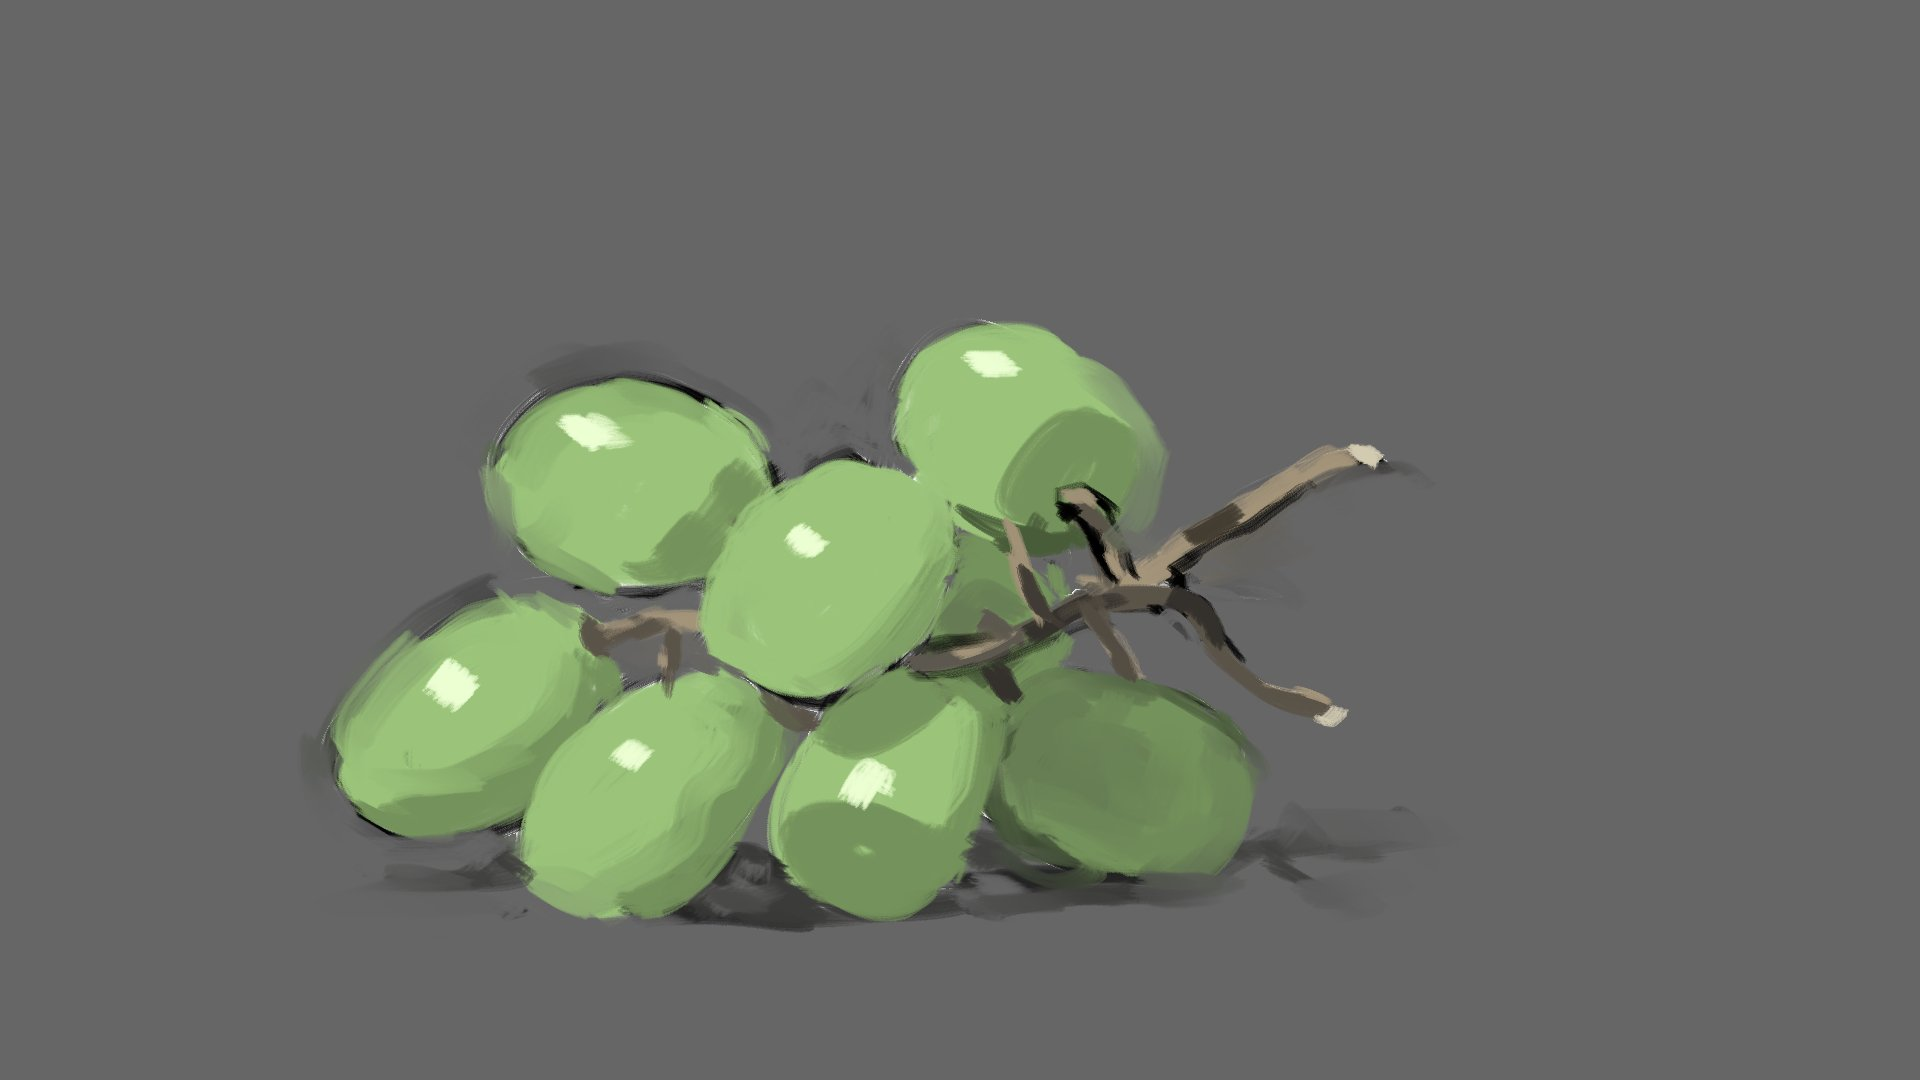
\includegraphics[scale = 0.1]{grapes.jpg}
    \caption{Some grapes}
    \label{}
\end{figure}

\section{The Cross Product}
While the dot product is used to take two equal-length sequences of numbers and return a single number,
we can use \textbf{the cross product} in order to multiply and get vectors in 3D.
\begin{figure}[h!]
    \centering
    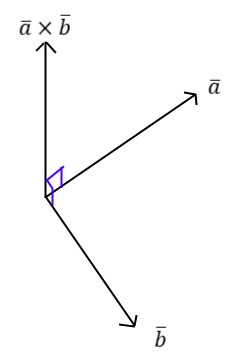
\includegraphics[scale=.5]{TripleProduct.png}
    \label{}
\end{figure}
\[\begin{bmatrix}
    i&j&k\\
    a&b&c\\
    d&e&f
\end{bmatrix}\begin{matrix}
    \leftarrow unit\\
    \leftarrow \vec{v}\\
    \leftarrow \vec{w}
\end{matrix}\]

\textbf{This method does not work in 2D.}
\subsection*{Example}
\[\vec{v}=(1,2,3) \;\;\; \vec{w}=(4,5,6) \]
\[\vec{v}\times \vec{w}=\begin{bmatrix}
    i&j&k\\
    1&2&3\\
    4&5&6
\end{bmatrix}=(2\cdot 6-3\cdot 5)\hat{i}-(1\cdot 6-3\cdot 4)\hat{j}+(1\cdot 5-2\cdot 4)\hat{k}\]
\[=-3\hat{i}+6\hat{j}-3\hat{k}\]
This gives us the direction of the cross product.


\subsection{Triple Product Formula}
We can find the product of three 3-dimensional vectors with the \textbf{triple product}
\[\vec{a}=(a_1,a_2,a_3)\;\;\; \vec{b}=(b_1,b_2,b_3)\;\;\; \vec{c}=(c_1,c_2,c_3)\]
\[\mbox{Triple Product}=(\vec{a}\times\vec{b})\cdot \vec{c}=\begin{bmatrix}
    a_1&a_2&a_3\\
    b_1&b_2&b_3\\
    c_1&c_2&c_3
\end{bmatrix}\]

3x3 Determinants equal zero if and only if the 3 row vectors lie on a single plane.

Because of this, $\vec{a}\times \vec{b}$ is orthogonal to the plane spanned by $\vec{a}\times \vec{b}$

$\vec{a}\times \vec{b}$ is orthogonal/perpendicular to both $\vec{a}$ and $\vec{b}$
\subsubsection*{Consequences}
\begin{enumerate}
    \item If $\vec{a}$ and $\vec{b}$ are co-linear (the same line through the origin), then $\vec{a}\times \vec{b}=(0,0,0)$
    \item If $\vec{a}$ and $\vec{b}$ are unit vectors, then $||\vec{a}\times \vec{b}||=\sin(\theta)$
    \item If $\vec{a}$ and $\vec{b}$ are perpendicular, then $||\vec{a}||\cdot ||\vec{b}||=||\vec{a}\times\vec{b}||$
\end{enumerate}
\section{Determinant Signs}
\subsection{2x2 Determinant Signs}
\begin{figure}[h!]
    \centering
    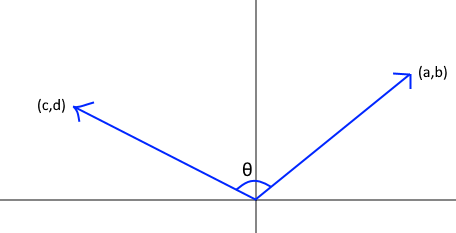
\includegraphics[scale=.5]{2x2DeterminantSign.png}
    \label{}
\end{figure}
If the angle from $(a,b)$ to $(c,d)$ $0\leq \theta\leq\pi$, then $\begin{bmatrix}
    a&b\\
    c&d
\end{bmatrix}\geq0$
\newline
If the angle from $(a,b)$ to $(c,d)$ $-\pi \leq \theta\leq 0$, then $\begin{bmatrix}
    a&b\\
    c&d
\end{bmatrix}\leq0$

\subsection{3x3 Determinant Signs}
\[\vec{a}=(a_1,a_2,a_3)\;\;\; \vec{b}=(b_1,b_2,b_3)\;\;\; \vec{c}=(c_1,c_2,c_3)\]

If the vectors $\vec{a},\vec{b},\vec{c}$ satisfy the right hand rule, then $\begin{bmatrix}
    a_1&a_2&a_3\\
    b_1&b_2&b_3\\
    c_1&c_2&c_3
\end{bmatrix}\leq 0$

If the vectors $\vec{a},\vec{b},\vec{c}$ fail the right hand rule (or satisfy the left hand rule), then $\begin{bmatrix}
    a_1&a_2&a_3\\
    b_1&b_2&b_3\\
    c_1&c_2&c_3
\end{bmatrix}\leq 0$
\begin{figure}[h!]
    \centering
    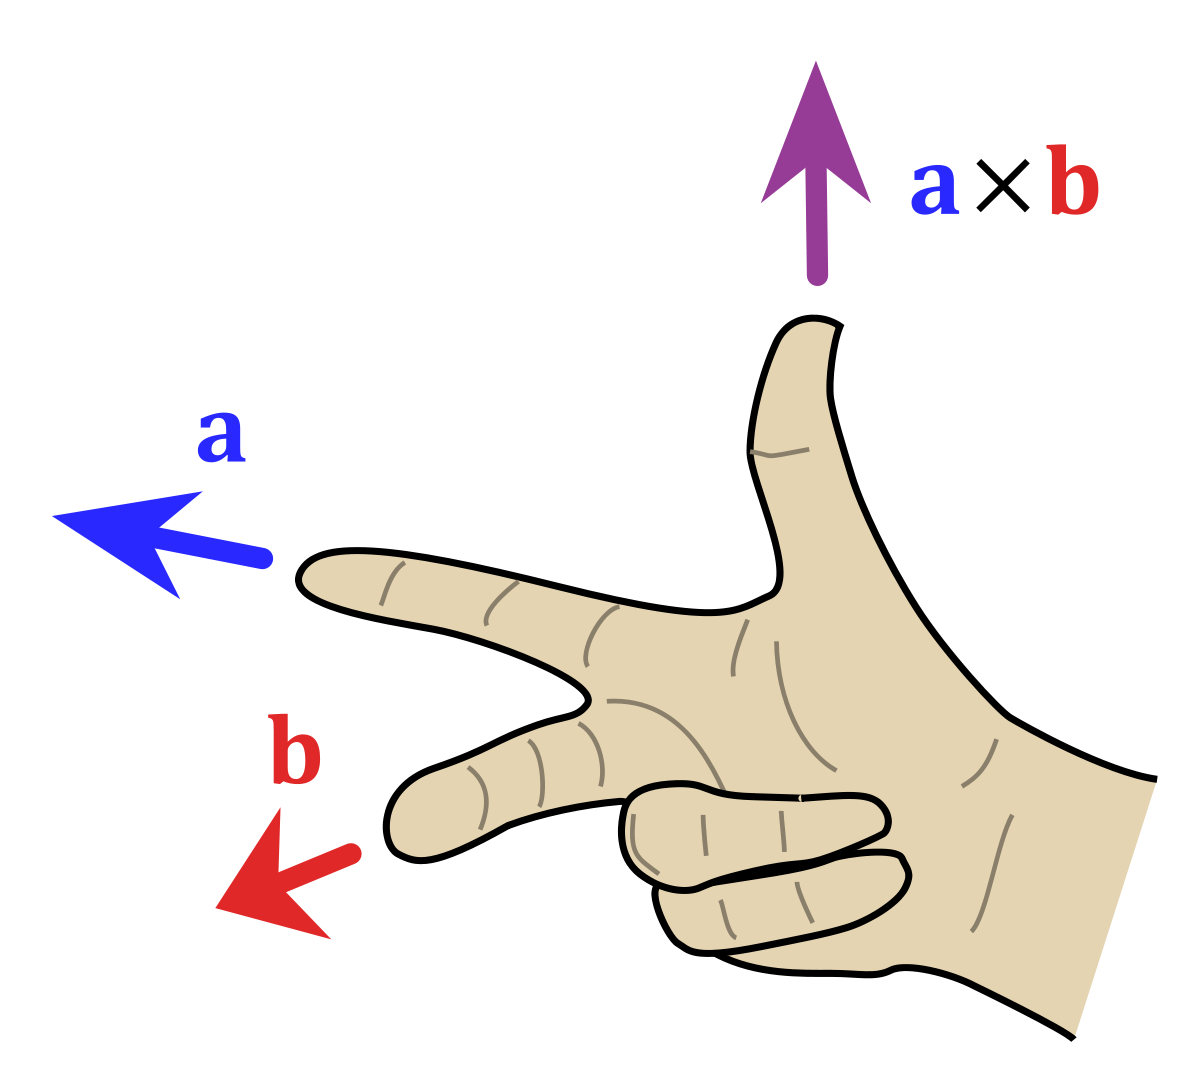
\includegraphics[scale=.1]{RightHandRule.png}
    \caption{The Right Hand Rule helps us find the direction of the cross product using two vectors}
    \label{}
\end{figure}
\newline
If $\vec{a}\times\vec{b}\neq(0,0,0)$, then $\vec{a},\vec{b},\vec{a}\times\vec{b}$ satisfy the right hand rule.

\begin{figure}[h!]
    \centering
    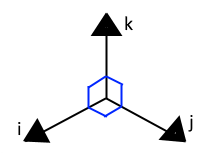
\includegraphics[scale=.5]{triplesign.png}
    \caption{}
    \label{}
\end{figure}
\[i×j=k\;\;\;j×k=i\;\;\;k×i=j\]
\[j×i=−k\;\;\;k×j=−i\;\;\;i×k=−j\]

\[i\times j=\begin{bmatrix}
    i&j&k\\
    1&0&0\\
    0&1&0
\end{bmatrix}=i(0)−j(0)+k(1⋅1−0⋅0)=k\]
\begin{figure}[h!]
    \centering
    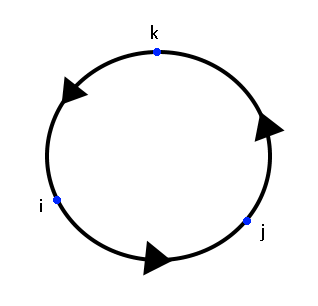
\includegraphics[scale=0.5]{circlesign.png}
    \caption{}
    \label{}
\end{figure}

\section{Properties of the Cross Product}
\begin{itemize}
    \item $\vec{a}\times\vec{b}=(0,0,0)$ if and only if $\vec{a}$ and $\vec{b}$ are parallel
    \item (Skew Symmetry) $\vec{a}\times\vec{b}=-\vec{a}\times\vec{b}$
    \item $\vec{a}\times (\vec{b}+\vec{c})=\vec{a}\times\vec{b}+\vec{a}\times\vec{c}$ and $(\vec{a}+\vec{b})\times\vec{c}=\vec{a}\times\vec{c}+\vec{b}\times\vec{c}$
    \item $(\alpha\vec{a})\times\vec{b}=\alpha(\vec{a}\times\vec{b})$
\end{itemize}
\subsection*{Warning}
The cross product is not associative, so
\[(\vec{a}\times\vec{b})\times\vec{c}\neq\vec{a}\times(\vec{b}\times\vec{c})\]
The cross product also does not interact well with the dot product (except for the triple product formula).
\subsection*{Exercise}
Compute $(0,0,1)\times(1,1,0)$ AND $(1,0,0)\times(1,1,0)$
\[(0,0,1)\times(1,1,0)=\begin{bmatrix}
    i&j&k\\
    0&0&1\\
    1&1&0
\end{bmatrix}=\hat{i}(0\cdot 0-1\cdot 1)-\hat{j}(0\cdot 0-1\cdot 1)+\hat{k}(0\cdot 1-0\cdot 1)=-\hat{i}+\hat{j}\]
\textbf{OR}
\[(0,0,1)=\hat{k}\;\;\;(1,1,0)=\hat{i}+\hat{j}\]
\[\hat{k}\times(\hat{i}+\hat{j})\]

\[(1,0,0)\times(1,1,0)=\begin{bmatrix}
    i&j&k\\
    1&0&0\\
    1&1&0
\end{bmatrix}=\hat{i}(0\cdot 0-0\cdot 1)-\hat{j}(1\cdot 0-1\cdot 0)+\hat{k}(1\cdot 1-1\cdot 0)=\hat{k}\]
\textbf{OR}
\[\hat{i}\times(\hat{i}+\hat{j})\]

\section{Equation of Planes}
\[\overbrace{Ax+By+Cz=0}^{(A,B,C)\cdot(x,y,z)}\]
\[P=\mbox{solution set}=\mbox{all the vectors perpendicular to }(A,B,C)\]

\subsection*{Solutions}
Call $(A,B,C)$ the normal vector denoted by $\bar{n}$
\newline
If \textit{P} is a plane with normal vector $\bar{n}$ containing $P_o=(x_o,y_o,z_o)$
\newline
Alternate Equations for Plane $P$
\[=\bar{n}\cdot(x-x_o,y-y_o,z-z_o)=0\]
\[=A(x-x_o)+B(y-y_o)+C(z-z_o)=0\]
\[=Ax+By+Cz+D=0\]
\[(D=-Ax_o-By_o-Cz_o)\]

\subsection*{Example}
Find the equation for the plane through $(1,1,0),(1,0,1),(0,1,1)$
\begin{figure}[h!]
    \centering
    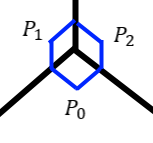
\includegraphics[scale=0.5]{planeExample.png}
    \caption{Needs a normal vector, given by $\vec{a}\times\vec{b}$}
    \label{}
\end{figure}

\subsubsection*{Consider}
\[\vec{a}=P_{1}-P_{0}=(0,-1,1)\]
\[\vec{b}=P_{2}-P_{0}=(-1,0,1)\]
\[(0,-1,1)\times(-1,0,1)=(-1,-1,-1)=(A,B,C)\]
\[P_o=(1,1,0)\mbox{ is a point in }P\]

Plane P can be found with
\[(A,B,C)\cdot (x-1,y-1,z-0)=0\]
\textbf{OR}
\[(-x+1,-y+1-z)=0\]
\[-x-y-z+2=0\;\;\; x+y+z=2\]

\section{Distance from a Point to a Plane}
Find the distance between the point $\vec{a}$ and the plane \textit{P}
\begin{figure}[h!]
    \centering
    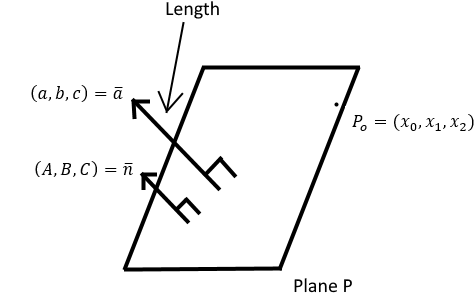
\includegraphics[scale=0.5]{pointToPlane.png}
    \label{}
\end{figure}

\subsection*{Equations}
\[\bar{n}\cdot((x,y,z)-P_o)=0\]
\textbf{OR}
\[\bar{n}\cdot((x-x_o,y-y_o,z-z_o)=0\]
\textbf{OR}
\[A(x-x_o)+B(y-y_o)+C(z-z_o)=0=Ax+By+Cz+D\]
\newline
We can find the line segment from $\vec{a}$ and the plane \textit{P} using the scalar multiple of the normal vector, $\bar{n}$
\newpage
The answer should be the length of the projection of $(\vec{a}-P_o)$ onto $\bar{n}$
\begin{figure}[h!]
    \centering
    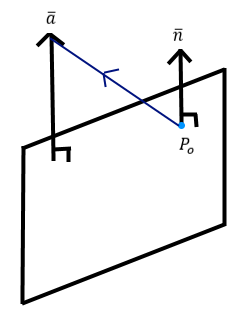
\includegraphics[scale=.6]{projectionExample.png}
    \label{}
\end{figure}
\[\overbrace{||{\frac{(\vec{a}-P_o)\cdot\bar{n}}{\vec{n}\cdot\vec{n}}\cdot\vec{n}}||}^{\mbox{The projection of $(\vec{a}-P_o)$ onto $\bar{n}$}}\]
\[=||\frac{((a,b,c)-(x_0,x_1,x_2))\cdot(A,B,C)}{(A,B,C)\cdot(A,B,C)}\cdot(A,B,C)||\]
\[=\frac{|Aa+Bb+Cc+D}{A^2+B^2+C^2}||\bar{n}||\]
\[=\frac{|Aa+Bb+Cc+D}{\sqrt{A^2+B^2+C^2}}\]
\newline
\[\overbrace{D=(x_0,x_1,x_2)\cdot(A,B,C)}^{\mbox{D is the collection of constants}}\]

\section{Multi-variable Functions}
We consider functions with domains/co-domains either $\mathbb{R},\; \mathbb{R}^2,\; \mathbb{R}^3$

\subsection*{Case 1}
A function with domains $\mathbb{R}$ and co-domains $\mathbb{R}$ 
\[f: \mathbb{R}\rightarrow\mathbb{R}^2\]
\begin{figure}[h!]
    \centering
    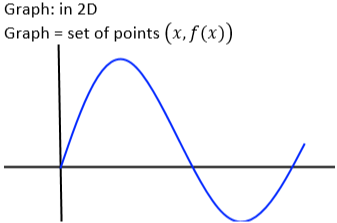
\includegraphics[scale=.5]{2DGraph.png}
    \caption{A Regular Real Function}
    \label{}
\end{figure}

\subsection*{Case 2}
\[\begin{matrix}
    f:\mathbb{R}\rightarrow\overbrace{\mathbb{R}^2}^{\mbox{2D Vector}}\\
    \mbox{\textbf{OR}}\\
    g:\mathbb{R}^2\rightarrow\overbrace{\mathbb{R}}^{\mbox{Real Number}}
\end{matrix}\begin{Bmatrix}
    \\
    \\
    \mbox{For these functions, we can still graph them}\\
    \\
    \\
\end{Bmatrix}\]

The graph of $f$ is the set of points $(x,f(x))$ in $\overbrace{\mathbb{R}^3}^{\mbox{3D Vector}}$

\subsubsection*{Example 1}
\[f(x)=(\cos(x),\sin(x))\]
Question: What is the range of the function?
\newline
Answer: The Unit Circle

\begin{figure}[h!]
    \centering
    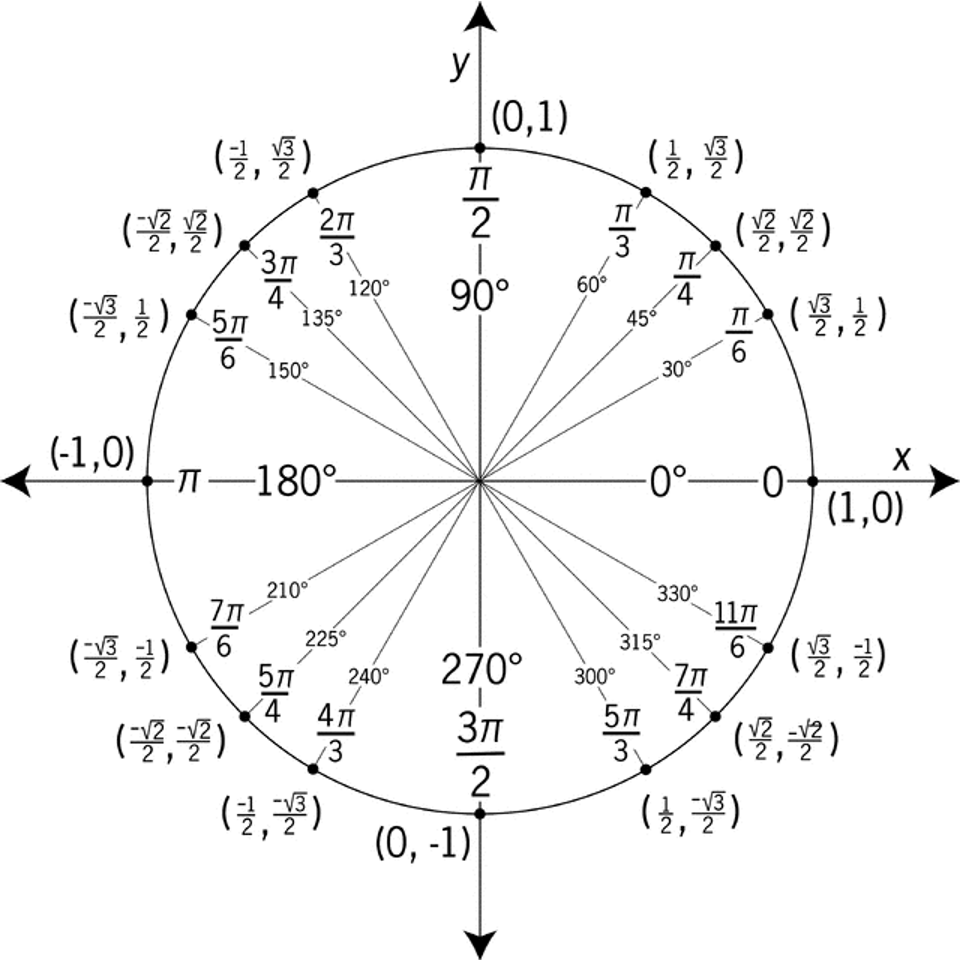
\includegraphics[scale=.1]{unitcircle.png}
    \label{}
\end{figure}
The graph of $f(x)=(\cos(x),\sin(y))$ creates a perfect spiral.
\begin{figure}[h!]
    \centering
    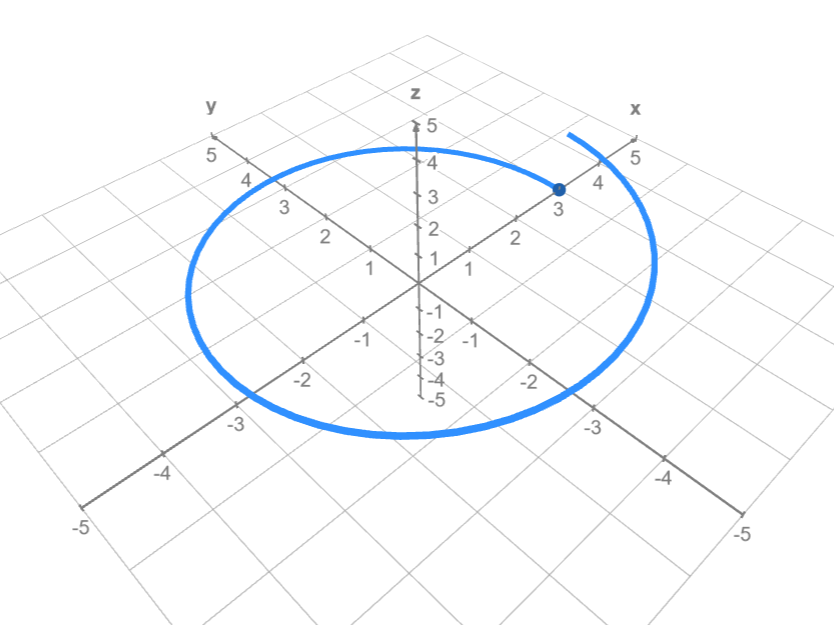
\includegraphics[scale=.3]{unitcirclespiral.png}
    \caption{}
    \label{}
\end{figure}

\[g:\mathbb{R}^2\rightarrow\mathbb{R}\]
The graph is a set of points in 3D of the form $(x,y,g(x,y))$
\newpage
\subsubsection*{Example 2}
\[g((x,y))=(x,y)\cdot(x,y)=x^2+y^2\]

The range of the function = All non-negative real numbers $\mathbb{R}$
\[(x,y)=(0,0)\]
This creates a surface
\begin{figure}[h!]
    \centering
    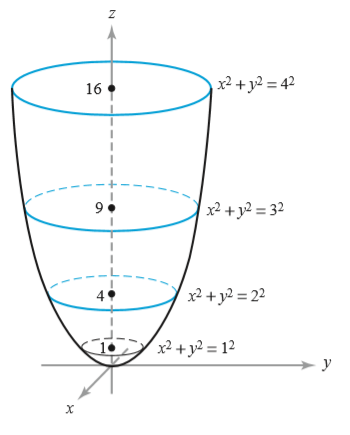
\includegraphics[scale=.5]{R2toR.png}
    \caption{}
    \label{}
\end{figure}

\subsection{Hard to Graph Functions}
Graphs are useful when the domain and co=domain have dimensions less than three. If $f:\mathbb{R}^3\rightarrow\mathbb{R}$ is a function, the level set with level $c$, where $c$ is a real number, is the subject of points in $\mathbb{R}$ that map to $c$
\subsubsection*{Example}
\[f:\mathbb{R}^3\rightarrow\mathbb{R}\]
\[(x,y,z)\rightarrow x^2+y^2+z^2=f(x,y,z)\]
\begin{figure}[h!]
    \centering
    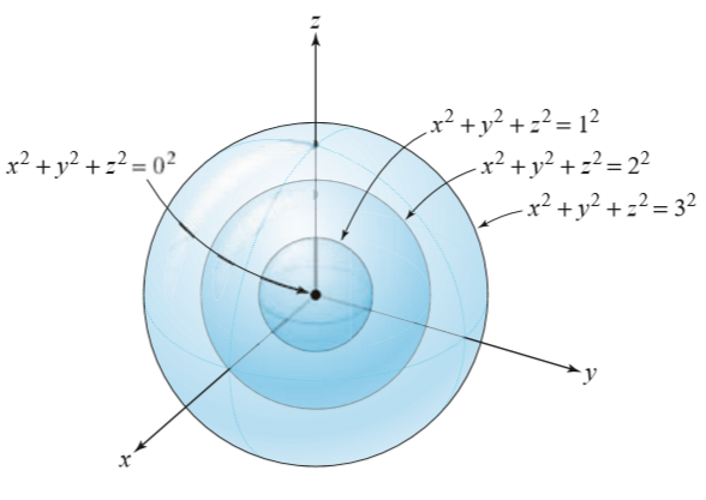
\includegraphics[scale=.3]{levelSets.png}
    \caption{Also known as level surfaces}
    \label{}
\end{figure}

\begin{itemize}
    \item Level 1
    \begin{itemize}
        \item A set with length = 1
        \item Sphere of radius $\sqrt{1}=1$
        \item Set of a unit vector
    \end{itemize}
    \item Level 2
    \begin{itemize}
        \item A set with length 2
        \item Sphere of radius $\sqrt{2}$
    \end{itemize}
\end{itemize}

\subsubsection*{Exercise}
\[g: \mathbb{R}^2 \rightarrow\mathbb{R}\]
\[(x,y)\rightarrow x\cdot y\]
Find the level sets with level -1, 0, 1

\begin{figure}[h!]
    \centering
    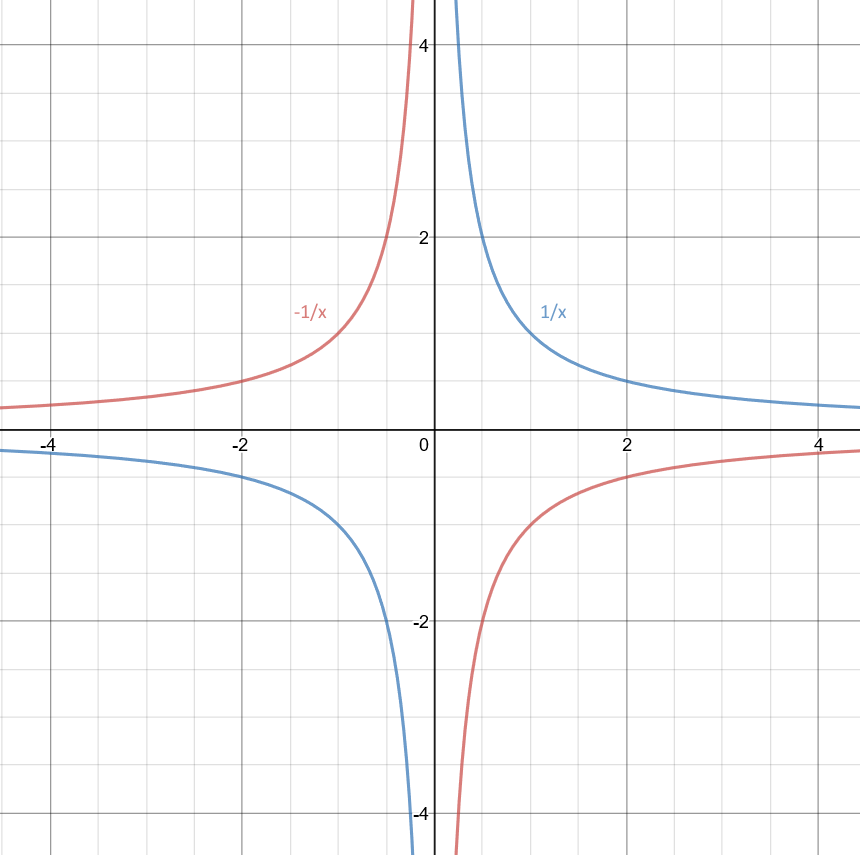
\includegraphics[scale=.2]{levelSetsNew.png}
    \label{}
\end{figure}
\begin{itemize}
    \item Level Set 0
    \begin{itemize}
        \item $xy=0$
        \item $x=0$ or $y=0$    
    \end{itemize}
    \item Level Set 1
    \begin{itemize}
        \item $xy=1$
        \item $y=\frac{1}{x}$    
    \end{itemize}
    \item Level Set -1
    \begin{itemize}
        \item $xy=-1$
        \item $y=-\frac{1}{x}$    
    \end{itemize}
\end{itemize}

\subsection{Taking Sections}
A section of a graph in 3D is the intersection of the graph with a plane.

\subsubsection*{Example}

\[h:\mathbb{R}^2\rightarrow\mathbb{R}\]
\[(x,y)\rightarrow x^{2}-y^{2}=h(x,y)\]

@ $x=0$
\[z=h(0,y)=-y^2\]
@$y=0$
\[z=h(x,0)=x^2\]


\begin{figure}[h!]
    \centering
    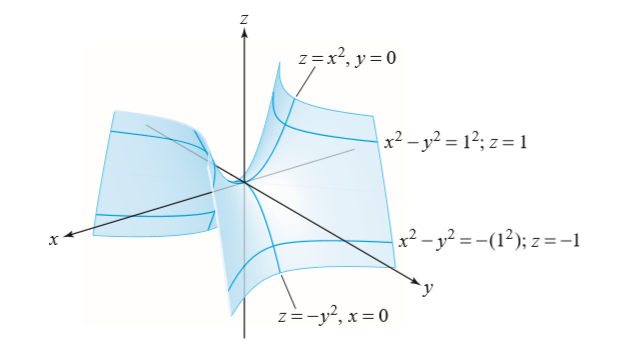
\includegraphics[scale=.5]{hyperbolicParabaloid.png}
    \label{}
\end{figure}



\end{document}